\documentclass[man,12pt,floatsintext]{apa7}
\usepackage[spanish,es-tabla]{babel}
\usepackage[utf8]{inputenc}
\usepackage{csquotes}   
\usepackage{amsmath}
\usepackage{graphicx}
\usepackage{float}
\usepackage[justification=centering]{caption}
\usepackage[nottoc]{tocbibind}
\usepackage{fancyhdr}
\usepackage[backend=biber, style=apa]{biblatex}
\usepackage{subcaption}
\usepackage{xcolor}
\usepackage{empheq}
\usepackage{tcolorbox}
\usepackage{cancel}
\usepackage{adjustbox}
\usepackage{geometry}
\usepackage{array}
\usepackage{booktabs}
\usepackage{caption}
\usepackage{placeins}
\usepackage{hyperref}
\usepackage{etoolbox}   % Siguiente pagina subsection
\pretocmd{\section}{\clearpage}{}{}
\geometry{left=35mm, right=25mm}
\captionsetup[figure]{position=top}

\hypersetup{
    colorlinks=true,
    linkcolor=black,   % ← índice, referencias internas
    urlcolor=blueS,    % ← enlaces web
    citecolor=black    % ← citas
}

\definecolor{blueS}{RGB}{0, 104, 204}
\addbibresource{bibliography.bib}

%%%%%%%%%%%%%%%%%%%%%%%%%%%%%%%%%
%   NUMERACIÓN DE SECCIONES     %
%%%%%%%%%%%%%%%%%%%%%%%%%%%%%%%%%
\setcounter{secnumdepth}{4}
\renewcommand{\sectionmark}[1]{\markboth{#1}{}}
\renewcommand{\thesection}{\arabic{section}}
\renewcommand{\thesubsection}{\thesection.\arabic{subsection}}
\renewcommand{\thesubsubsection}{\thesubsection.\arabic{subsubsection}}

%%%%%%%%%%%%%%%%%%%%%%%%%%%%%%%%
%  ENCABEZADOS Y PIE DE PÁGINA %
%%%%%%%%%%%%%%%%%%%%%%%%%%%%%%%%
\newcommand{\aplicarEstilo}{
  \fancyhf{}
  \fancyfoot[L]{Universidad Mayor de San Simón}
  \fancyfoot[R]{\thepage}
  \fancyhead[L]{\nouppercase{\leftmark}}
  \renewcommand{\headrulewidth}{0.4pt}
  \renewcommand{\footrulewidth}{0.4pt}
  \setlength{\headheight}{16pt}
}

% chktex-file 1
\fancypagestyle{cuerpo}{
  \aplicarEstilo
}

\fancypagestyle{plain}{
  \aplicarEstilo
}

\begin{document}
\pagestyle{fancy}
\aplicarEstilo

\fancypagestyle{plain}{
  \aplicarEstilo
}

\clearpage
\newpage

%%%%%%%%%%%%%
%  CARÁTULA %
%%%%%%%%%%%%%
\begin{titlepage}
\thispagestyle{empty}
\begin{center}
  
\includegraphics[width=4cm]{images/cover/logoEscudoUmss.png}\\[0.1cm]
  {\normalsize \textbf{UNIVERSIDAD MAYOR DE SAN SIMÓN}}\\[0.1cm]
  {\normalsize FACULTAD DE CIENCIAS Y TECNOLOGÍA}\\[0.3cm]
  {\Large \textbf{PRÁCTICA DE FÍSICA GENERAL}}\\[0.3cm]
  {\normalsize \textbf{GRUPO X}}
\end{center}

\vspace{0.4cm}
\noindent\textbf{Integrantes:}\\[0.10cm]
Cabrera Sejas Alejandra Alicia\\
Flores Vallejos Jose Gabriel\\
Gutierrez Mollo Adriana\\
Paucara Gutierrez Kevin Willy\\
Quiñones Arias Erick\\
Serna Mesa Evelio

\vspace{0.2cm}
\noindent\textbf{Docente:}\\[0.10cm]
Lic. C. Mamani Luis Jose

\vspace{0.2cm}
\noindent\textbf{Materia:}\\[0.10cm]
Física General

\vspace{0.2cm}
\noindent\textbf{Carrera:}\\[0.10cm]
Ing. Informática

\begin{center}
  {\small \today}
\end{center}
\end{titlepage}
\newpage

%%%%%%%%%%%%%%%%%%%
%  ÍNDICE GENERAL %
%%%%%%%%%%%%%%%%%%%
\tableofcontents
\newpage
\listoffigures
\newpage
\listoftables
\newpage

%%%%%%%%%%%%%%%%%%
%  MARCO TEÓRICO %
%%%%%%%%%%%%%%%%%%
\section{Introducción}
La presente práctica de Física General tiene como propósito el estudio y análisis del movimiento 
de los cuerpos a través de los conceptos fundamentales de la cinemática. En este contexto, 
se abordan magnitudes físicas como la posición, el desplazamiento, la velocidad y la aceleración, 
las cuales permiten describir el comportamiento de un objeto en función del tiempo 
sin considerar las causas que originan dicho movimiento.\\
\vspace{10pt}

Asimismo, se desarrollan y aplican los modelos matemáticos correspondientes al Movimiento Rectilíneo Uniforme (MRU), 
al Movimiento Rectilíneo Uniformemente Acelerado (MRUA) 
y a la caída libre, estableciendo relaciones entre las variables físicas involucradas. 
El uso del cálculo diferencial e integral permite una comprensión más profunda de estos fenómenos, 
facilitando la obtención de ecuaciones que describen el movimiento de manera rigurosa.\\
\vspace{10pt}

Finalmente, se complementa el análisis teórico mediante el uso de herramientas tecnológicas, 
como simuladores, que permiten visualizar e interpretar gráficamente los resultados obtenidos, 
fortaleciendo así la comprensión conceptual y la validación de los procedimientos desarrollados.
\section{Objetivos}

\subsection{Objetivo General}

Analizar y comprender el movimiento de los cuerpos mediante el estudio de la cinemática, 
aplicando modelos matemáticos y herramientas de cálculo para describir, interpretar y resolver 
problemas relacionados con el Movimiento Rectilíneo Uniforme (MRU), el Movimiento Rectilíneo 
Uniformemente Acelerado (MRUA) y la caída libre (MVCL), así como desarrollar la simulación de un 
caso de MRUA mediante el uso del software GeoGebra.

\subsection{Objetivos Específicos}

\begin{itemize}
    \item Describir las magnitudes fundamentales de la cinemática, tales como posición, desplazamiento, velocidad y aceleración.
    \item Analizar las características del Movimiento Rectilíneo Uniforme (MRU) y del Movimiento Rectilíneo Uniformemente Acelerado (MRUA).
    \item Aplicar conceptos de cálculo diferencial e integral en la obtención de ecuaciones de movimiento.
    \item Estudiar el fenómeno de la caída libre considerando la aceleración de la gravedad.
    \item Resolver problemas físicos mediante el uso de ecuaciones cinemáticas.
    \item Utilizar herramientas tecnológicas para la simulación y verificación de los resultados obtenidos.
\end{itemize}
\section{Cinemática}
La cinemática es la rama de la física que estudia el movimiento de los cuerpos sin considerar las causas que lo producen.

\begin{figure}[H]
    \centering
    \captionsetup{width=0.6\textwidth}
    \caption{Gráfica posición-tiempo}
    \adjustbox{margin={0pt 5pt 0pt 0pt}}{
        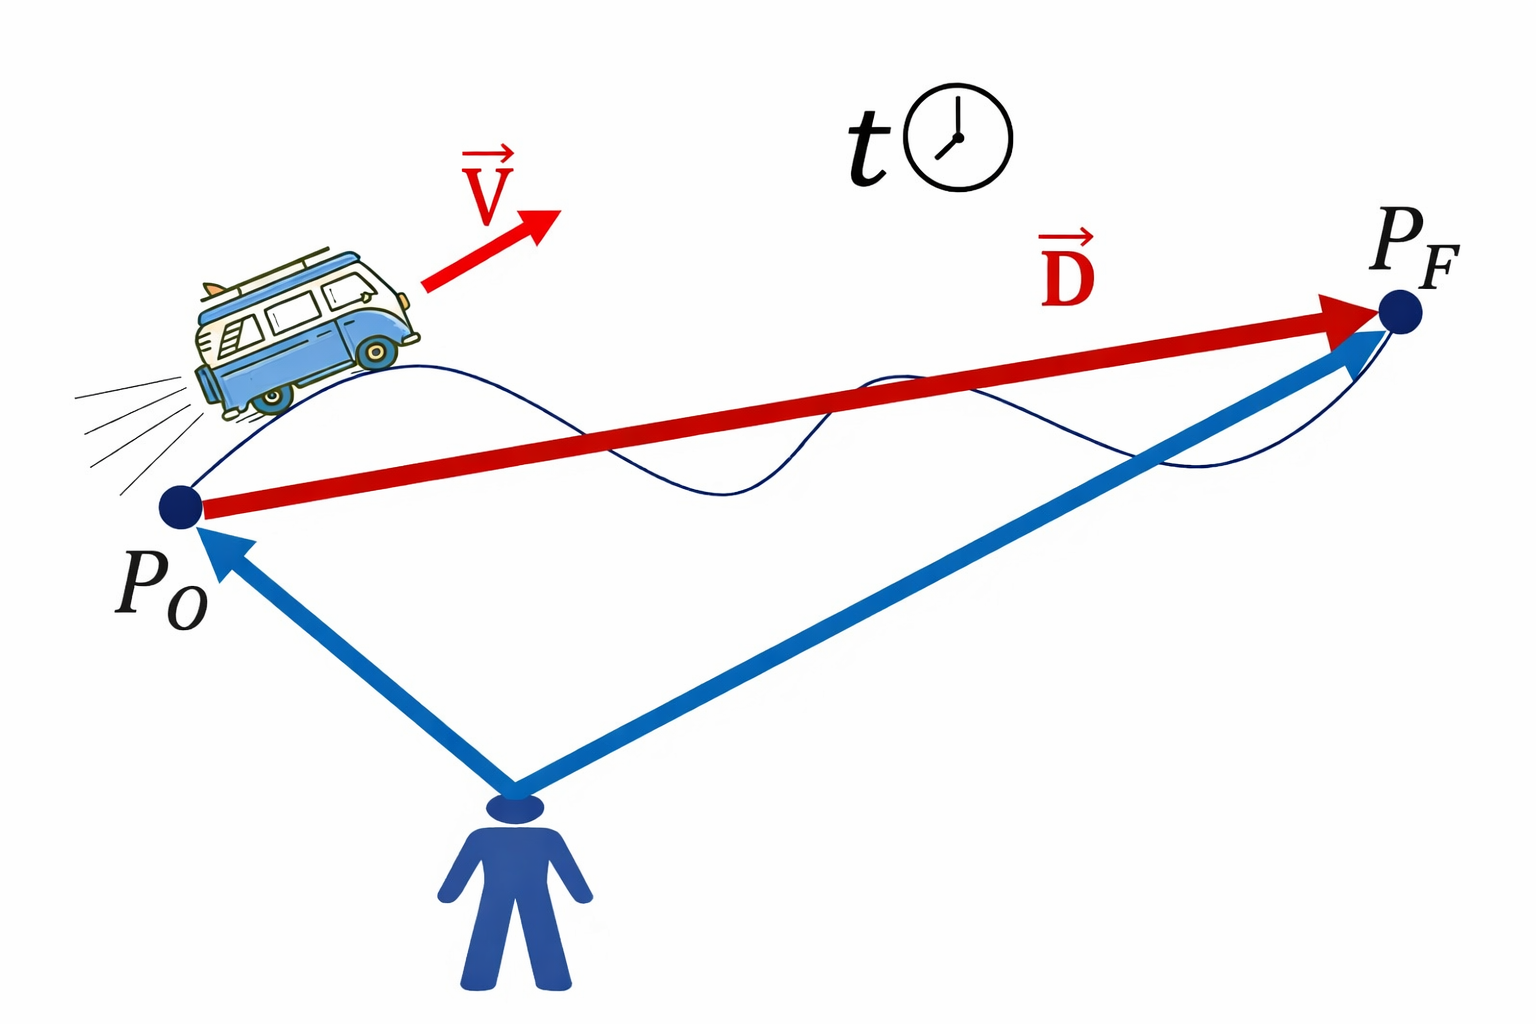
\includegraphics[width=0.6\textwidth]{images/cinematicImages/cinematic.png}
    }
    \caption*{Nota: Representa la relación entre posición y tiempo en el movimiento de un cuerpo.} 
\end{figure}

\vspace{-20pt}

\subsection{Sistema de referencia}
Es el marco o conjunto de coordenadas desde el cual un observador describe la posición y el movimiento de un objeto. Permite establecer medidas de distancia, dirección y tiempo.

\begin{figure}[H]
    \centering
    \captionsetup{width=0.6\textwidth}
    \caption{Sistema de referencia}
    \adjustbox{margin={0pt 10pt 0pt 0pt}}{
        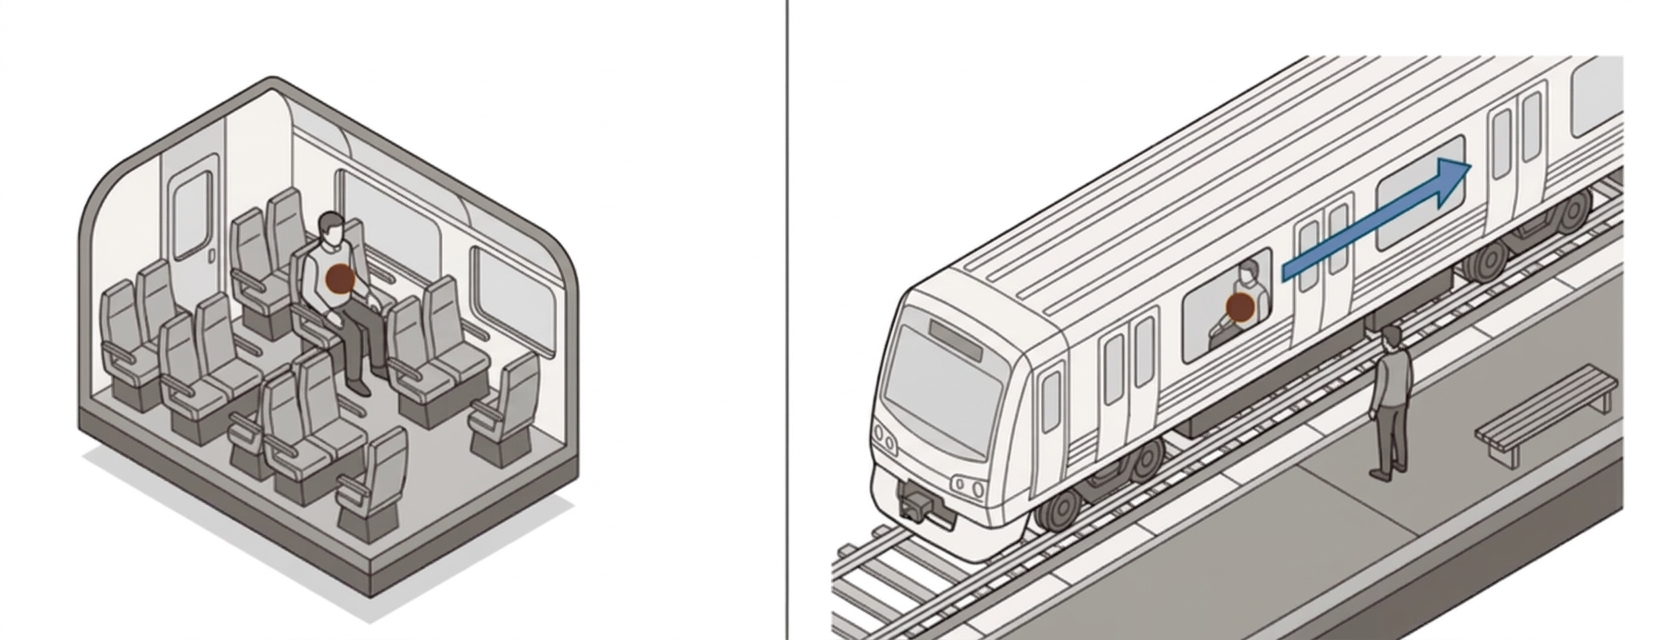
\includegraphics[width=0.7\textwidth]{images/cinematicImages/referenceSystem.png}
    }
    \caption*{Nota: Sistema de referencia desde el observador que describe la posición y el movimiento de un objeto. }
\end{figure}

\vspace{-20pt}

\subsubsection{Observador interno}
Es aquel que se encuentra dentro del sistema en movimiento, es decir, forma parte del cuerpo que se desplaza. Desde su perspectiva, los objetos que se mueven junto a él parecen estar en reposo, mientras que los elementos externos aparentan moverse en sentido contrario.

\subsubsection{Observador externo}
Es aquel que se encuentra fuera del sistema en movimiento, observando el desplazamiento desde un punto fijo. Desde su perspectiva, puede apreciar con claridad la trayectoria, la velocidad y los cambios de posición del cuerpo en movimiento.

\subsection{Posición}
La posición de un objeto indica su ubicación en el espacio respecto a un punto del sistema de referencia (origen). Se representa generalmente con la variable $x$ para el caso unidimensional.

\begin{itemize}
    \item \textbf{En una dimensión (1D):} la posición se describe mediante una sola coordenada, generalmente $x$, que indica la distancia (con signo) respecto al origen.
    \item \textbf{En dos dimensiones (2D):} la posición se describe mediante un vector $\vec{r}$ compuesto por dos coordenadas, $x$ e $y$, que determinan la ubicación del objeto en el plano.
\end{itemize}

\begin{figure}[H]
    \centering
    \captionsetup{width=0.6\textwidth}
    \caption{Posición de un cuerpo en una dimensión}
    \includegraphics[width=0.7\linewidth]{images/cinematicGraphics/1DPosition.jpg}
    \caption*{Nota: Representación de la posición de un cuerpo en un sistema unidimensional. }
\end{figure}

\vspace{-60pt}

\begin{align*}
    \Aboxed{\vec{r} = x_0(\pm \hat{\imath})}
\end{align*}

\begin{figure}[H]
    \centering
    \captionsetup{width=0.6\textwidth}
    \caption{Posición de un cuerpo en dos dimensiones}
    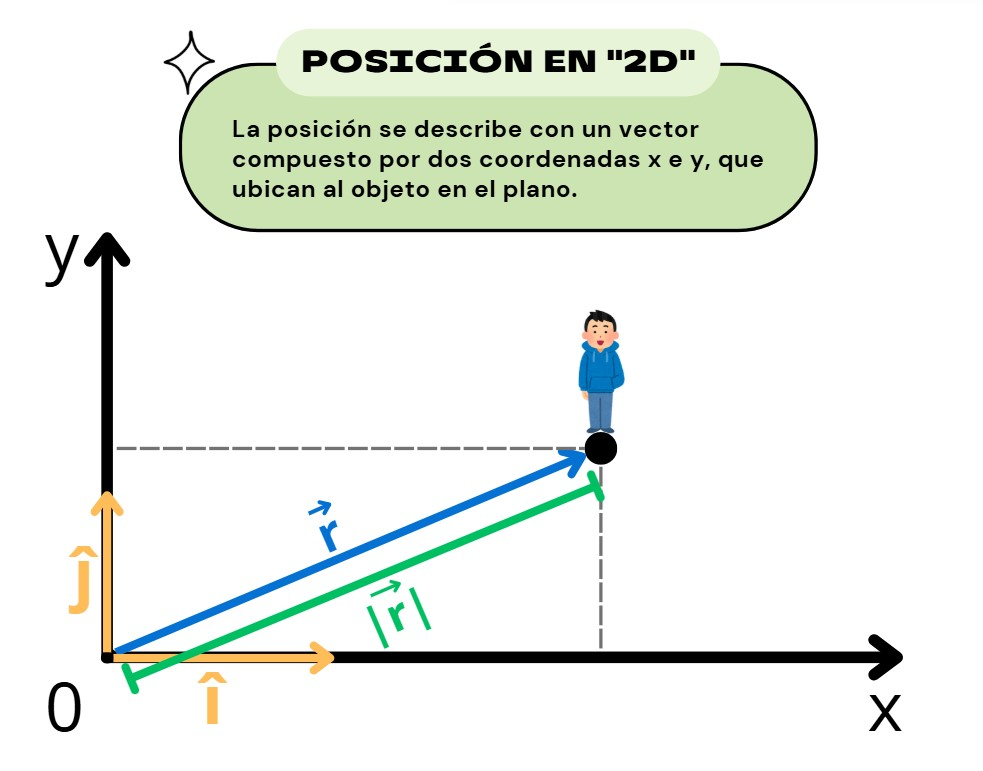
\includegraphics[width=0.7\linewidth]{images/cinematicGraphics/2DPosition.jpg}
    \caption*{Nota: Representación de la posición de un cuerpo en un plano bidimensional. }
\end{figure}

\vspace{-60pt}

\begin{align*}
    \Aboxed{\vec{r} = x\hat{\imath} + y\hat{\jmath}}\\
    \Aboxed{|\vec{r}| = \sqrt{x^2 + y^2}}
\end{align*}

\vspace{-20pt}

\[
[\vec{r}\,] = [\mathrm{m}] \quad \text{S.I.} 
\]

\subsection{Desplazamiento}
El desplazamiento es la variación de posición de un objeto entre dos instantes de tiempo.

\begin{figure}[H]
    \centering
    \captionsetup{width=0.5\textwidth}
    \caption{Desplazamiento en dos dimensiones}
    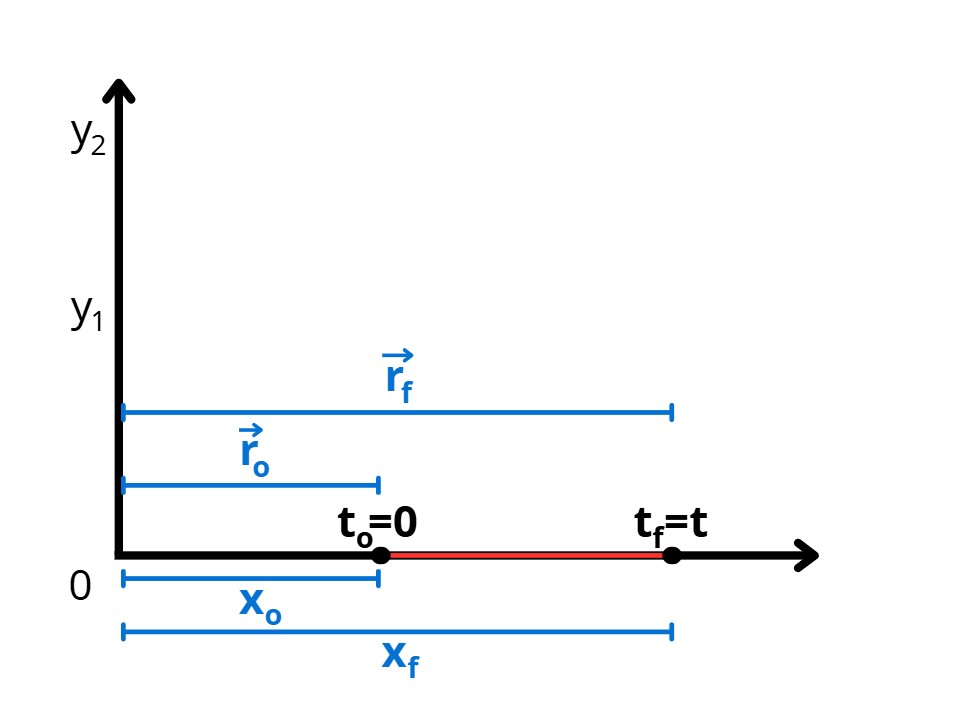
\includegraphics[width=0.7\linewidth]{images/cinematicGraphics/1DDisplacement.jpg}
    \caption*{Nota: Representación del desplazamiento de un cuerpo en un plano bidimensional. }
\end{figure}

\vspace{-60pt}

\begin{align}
    \Aboxed{\Delta \vec{x} = \vec{x}_f - \vec{x}_o}
\end{align}

\begin{figure}[H]
    \centering
    \captionsetup{width=0.5\textwidth}
    \caption{Desplazamiento en dos dimensiones}
    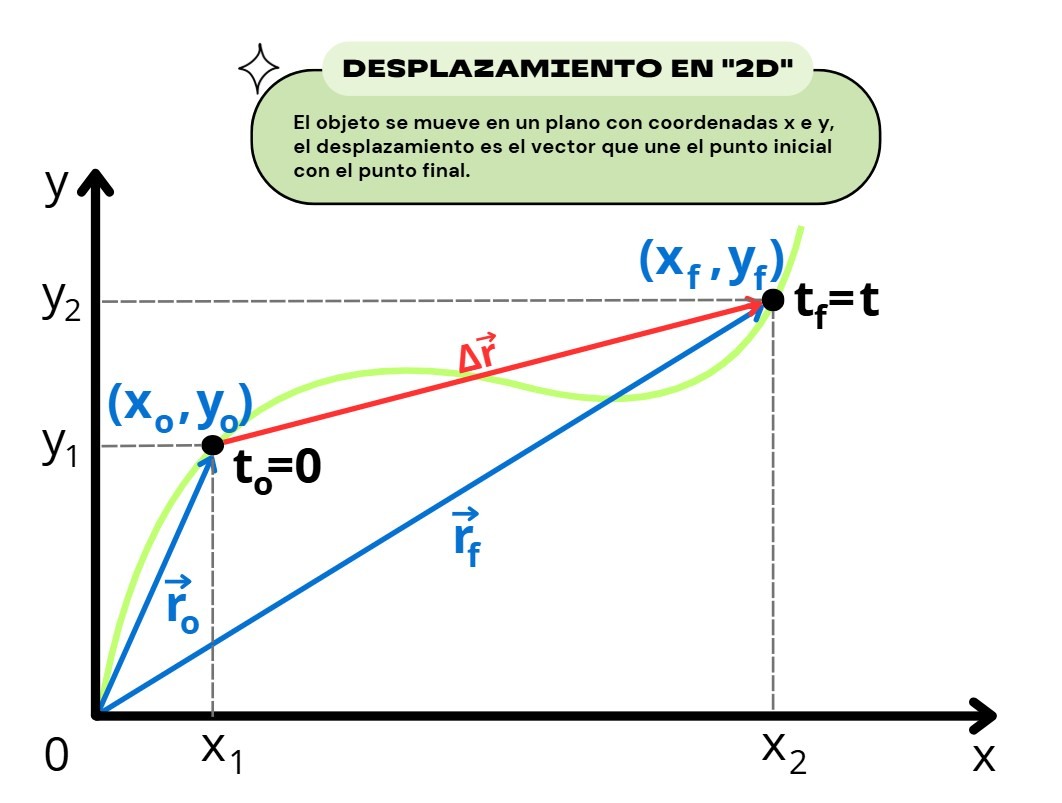
\includegraphics[width=0.7\linewidth]{images/cinematicGraphics/2DDisplacement.jpg}
    \caption*{Nota: Representación del desplazamiento de un cuerpo en un plano bidimensional. }
\end{figure}

\vspace{-60pt}

\begin{align}
    \Aboxed{\Delta \vec{r} = \vec{r}_f - \vec{r}_o}
\end{align}
\begin{align*}
    \vec{r}_o = x_o \hat{\imath} + y_o \hat{\jmath}\\
    \vec{r}_f = x_f \hat{\imath} + y_f \hat{\jmath}
\end{align*}

\vspace{-20pt}

\[
[\Delta \vec{r}\,] = [\mathrm{m}] \quad \text{S.I.} 
\]

Donde $x_f$ es la posición final y $x_0$ es la posición inicial.\\
El desplazamiento puede ser positivo, negativo o cero.

\subsection{Velocidad y rapidez}

\subsubsection{Velocidad}
La velocidad es una magnitud vectorial que expresa la variación de posición por unidad de tiempo. A diferencia de la rapidez, considera la dirección y el sentido del movimiento.

\begin{figure}[H]
    \centering
    \captionsetup{width=0.5\textwidth}
    \caption{Vector velocidad}
    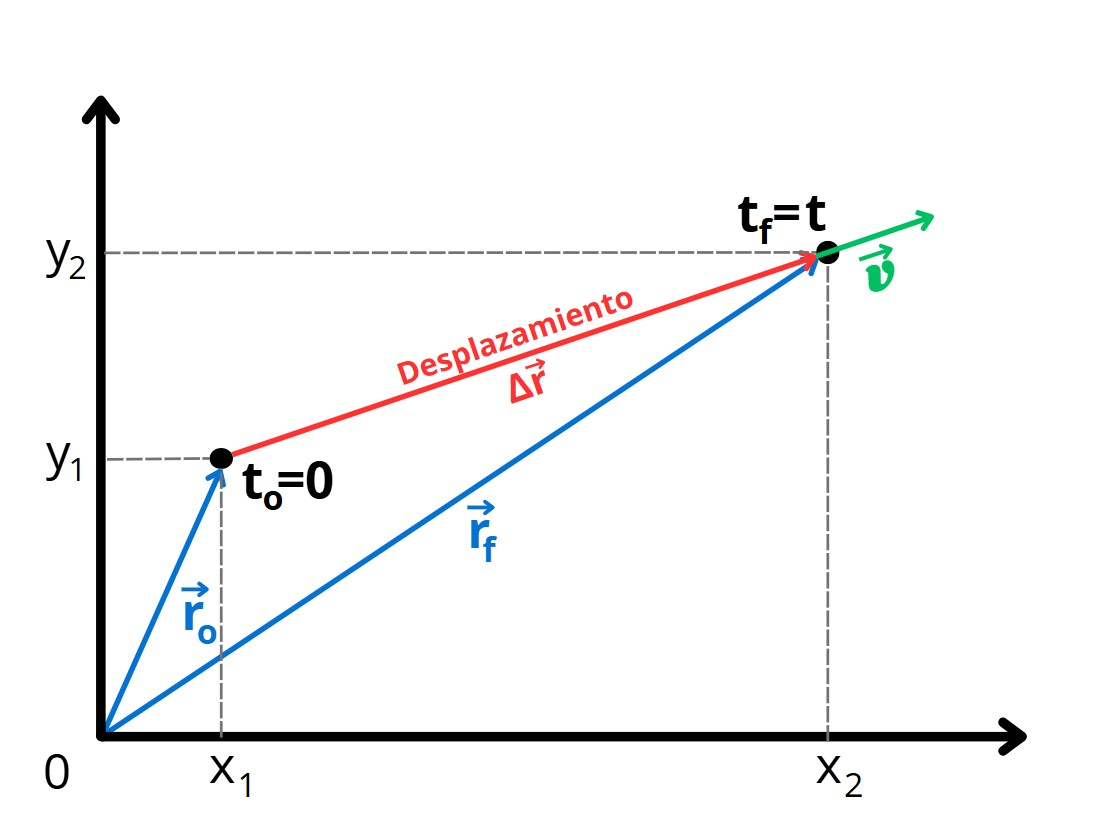
\includegraphics[width=0.5\textwidth]{images/cinematicGraphics/speedV.jpg}
    \caption*{Nota: Representación del vector velocidad, dirección y sentido en el plano.}
\end{figure}

\vspace{-40pt}
\[
\text{velocidad} = \frac{\text{desplazamiento}}{t} = \frac{\Delta{x}}{t}
\]

\vspace{-20pt}

\begin{align*}
    \Aboxed{\displaystyle {v} = \frac{\Delta x}{t}}
\end{align*}

\subsubsection{Rapidez}

La rapidez es una magnitud escalar que indica qué tan rápido se mueve un objeto.

\begin{figure}[H]
    \centering
    \captionsetup{width=0.5\textwidth}
    \caption{Magnitud de la velocidad}
    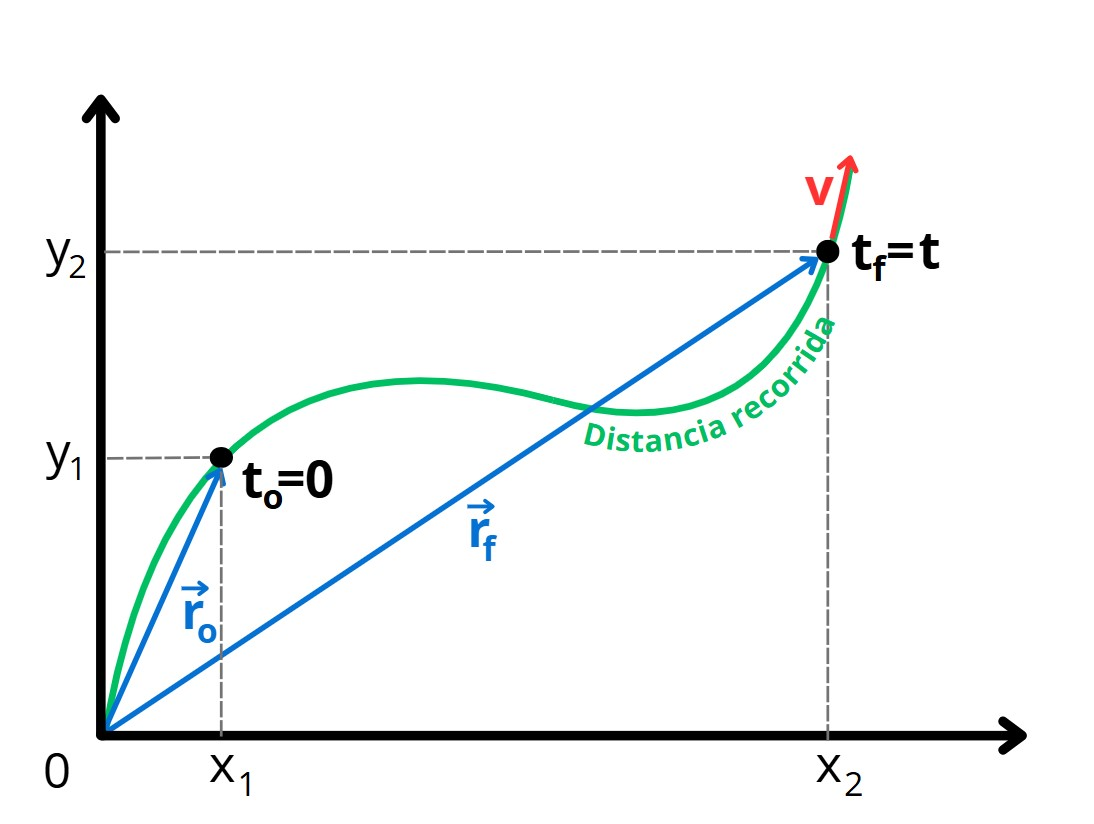
\includegraphics[width=0.5\textwidth]{images/cinematicGraphics/speedR.jpg}
    \caption*{Nota: Representación de la rapidez como el valor escalar de la velocidad}
\end{figure}

\vspace{-40pt}

\[
\text{rapidez} = \frac{\text{distancia recorrida}}{t} = \frac{\text{d}}{t}
\]

\vspace{-20pt}

\begin{align*}
    \Aboxed{\displaystyle \text{v} = \frac{\text{d}}{t}}
\end{align*}

\subsection{Velocidad media e instantánea}

\subsubsection{Velocidad media}
La velocidad media es una magnitud vectorial que se define como el cambio de posición (desplazamiento) dividido entre el intervalo de tiempo en el que ocurre ese cambio.

\begin{figure}[H]
    \captionsetup{width=0.5\textwidth}
    \caption{Velocidad media en un intervalo de tiempo}
    \centering
    \includegraphics[width=0.6\textwidth]{images/cinematicGraphics/averageSpeed.jpg}
    \caption*{Nota: Representación del desplazamiento en un intervalo de tiempo.}
\end{figure}

\vspace{-50pt}

\begin{align}
    \Aboxed{\displaystyle \vec{v}_m = \frac{\Delta \vec{r}}{\Delta t}} = \frac{\vec{r}_f - \vec{r}_o}{\vec{t}_f - \vec{t}_o}
\end{align}

\vspace{-20pt}

\[
[\vec{v}_m\,] = [\frac{m}{s}] \quad \text{S.I.} 
\]

\subsubsection{Velocidad instantánea}
La velocidad instantánea es la velocidad de un objeto en un instante preciso de tiempo. Se obtiene como el límite de la velocidad media cuando el intervalo de tiempo tiende a cero.\\
Este límite es lo que en cálculo se conoce como la derivada de la posición respecto al tiempo.
\begin{figure}[H]
    \centering
    \captionsetup{width=0.5\textwidth}
    \caption{Velocidad instantánea en un punto de la trayectoria}
    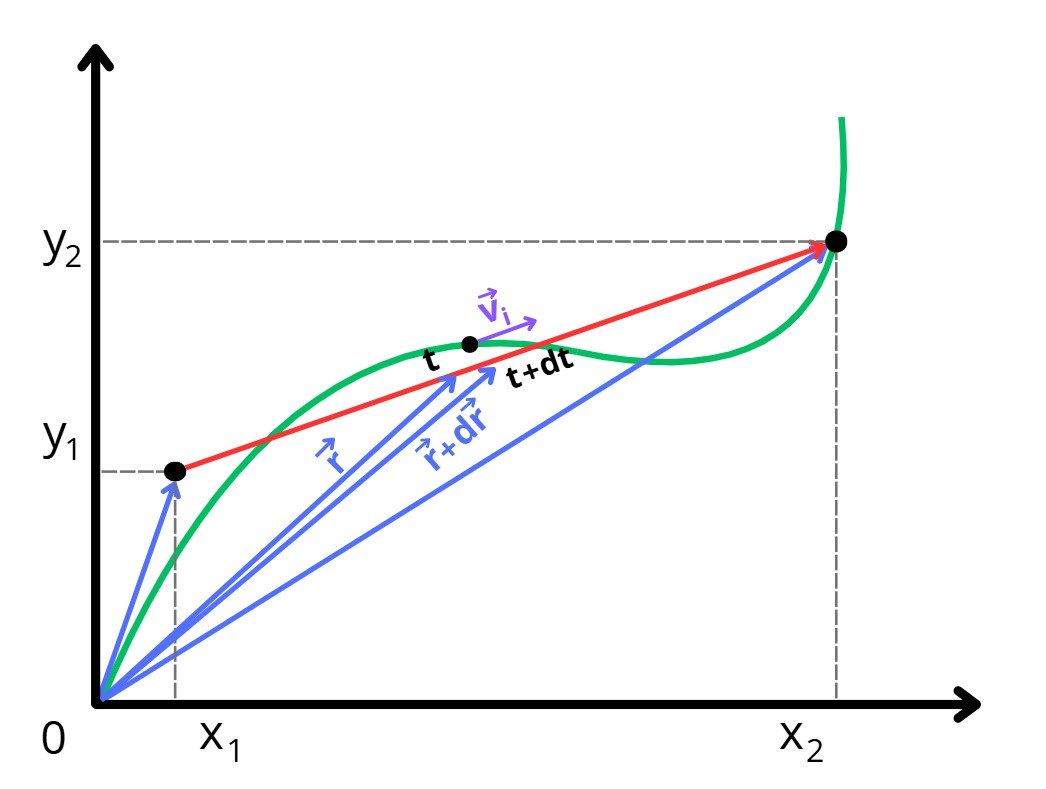
\includegraphics[width=0.6\textwidth]{images/cinematicGraphics/instantSpeed.jpg}
    \caption*{Representación de la velocidad instantánea como la pendiente de la curva posición-tiempo en un punto específico.}
\end{figure}

\vspace{-40pt}

\begin{align}
    \Aboxed{\vec{v} = \lim_{\Delta t \to 0} \frac{\Delta \vec{r}}{\Delta t}} = \frac{d\vec{r}}{dt}
\end{align}

\vspace{-20pt}

\[
[\vec{v}\,] = [\frac{m}{s}] \quad \text{S.I.} 
\]

\subsubsection{Ejemplo}

Determinar la velocidad instantánea de la partícula.

\begin{figure}[H]
    \centering
    \captionsetup{width=0.5\textwidth}
    \caption{Velocidad instantánea en un punto}
    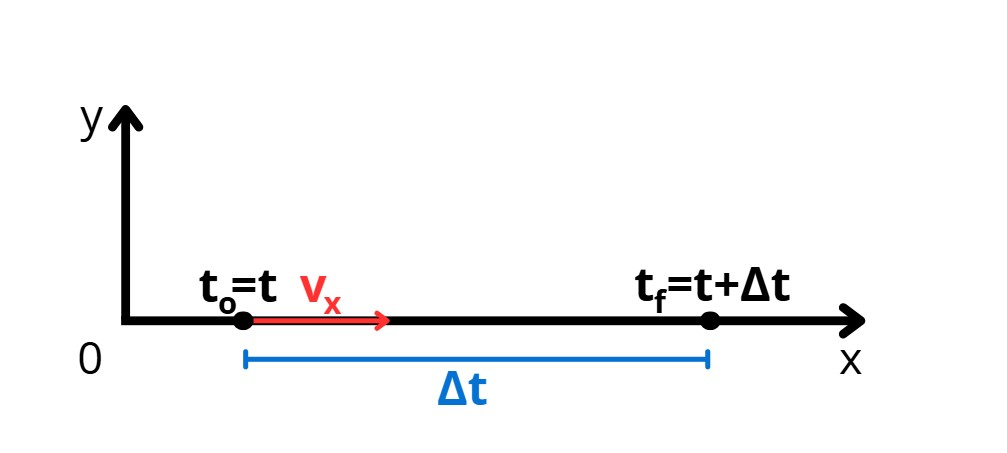
\includegraphics[width=0.6\textwidth]{images/demonstrations/example1.jpg}
    \caption*{Nota: Representación de la velocidad instantánea en un punto de la trayectoria.}
\end{figure}
\vspace{-40pt}

% chktex-file 3
\begin{align*}
&\textbf{Comprobación usando integrales:} \\
    \vec{v_x} &= \lim_{\Delta t \to 0} \frac{\Delta \vec{x}}{\Delta t} \\
    \vec{v_x} &= \lim_{\Delta t \to 0} \frac{x_f(t_f) - x_o(t_o)}{\Delta t} \\
&\text{Considerar } x(t) = t^2: \\    
    v_x &= \lim_{\Delta t \to 0} \frac{t_f^2 - t_o^2}{\Delta t} \\
    v_x &= \lim_{\Delta t \to 0} \frac{(t + \Delta t)^2 - t^2}{\Delta t} \\
    v_x &= \lim_{\Delta t \to 0} \frac{\cancel{t^2} + 2t\Delta t + (\Delta t)^2 - \cancel{t^2}}{\Delta t} \\
    v_x &= \lim_{\Delta t \to 0} \frac{\cancel{\Delta t}(2t + \Delta t)}{\cancel{\Delta t}} \\
    v_x &= \lim_{\Delta t \to 0} (2t + \cancel{\Delta t}) \\
    \Aboxed{v_x &= 2t} \\
\end{align*}
\begin{align*}
&\textbf{Comprobación usando derivada:} \\
    v_x &= \frac{dx(t)}{dt} \\
    v_x &= \frac{d}{dt}(t^2) \\
    v_x &= 2t^{2-1} \\
    \Aboxed{v_x &= 2t}
\end{align*}

\vspace{-30pt}

\[
\Rightarrow \quad \text{Ambos métodos coinciden.}
\]

\subsection{Aceleración media e instantánea}

\begin{figure}[H]
    \centering
    \captionsetup{width=0.5\textwidth}
    \caption{Aceleración media en un intervalo de tiempo}
    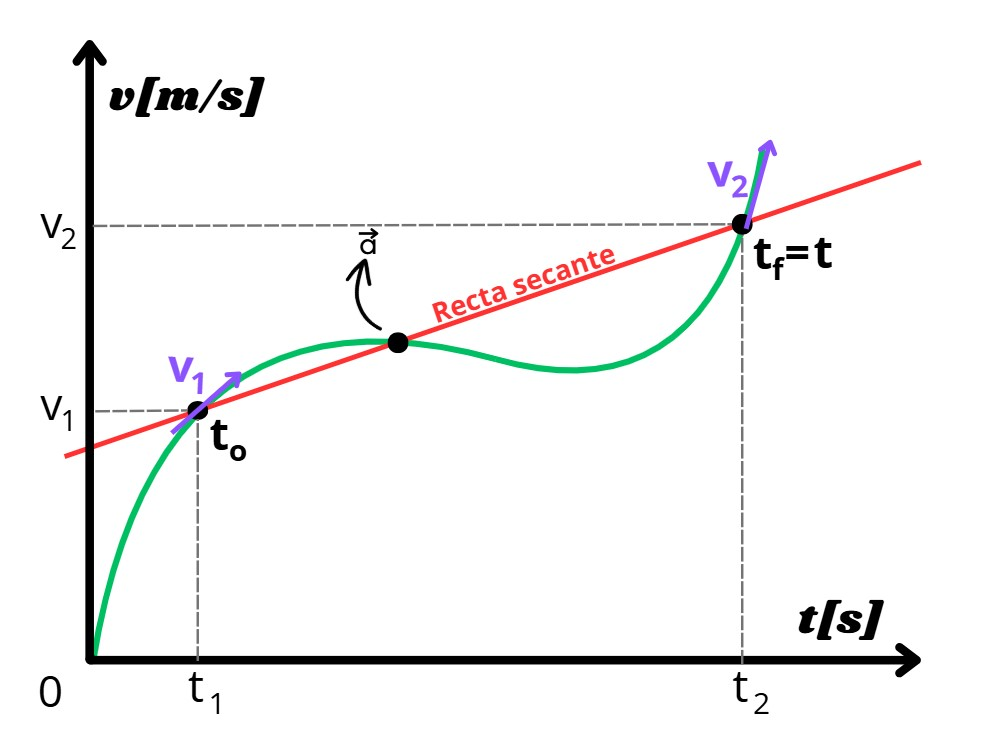
\includegraphics[width=0.6\textwidth]{images/cinematicGraphics/averageAcceleration.jpg}
    \caption*{Representación de la aceleración como cambio de la velocidad en el tiempo.}
\end{figure}

\vspace{-40pt}

\[
[a] = [\frac{m/s}{s}] = [\frac{m}{s^2}]  \quad \text{S.I.} 
\]

\subsubsection{Aceleración media}
La aceleración media mide la variación de la velocidad en un intervalo de tiempo determinado:
\vspace{-20pt}

\begin{align}
    \Aboxed{\displaystyle \vec{a}_m = \frac{\Delta \vec{v}}{\Delta t}} = \frac{v_f - v_0}{t_f - t_0}
\end{align}

\subsubsection{Aceleración instantánea}

La aceleración instantánea es la aceleración de un objeto en un instante preciso. Se define como el límite de la aceleración media cuando el intervalo de tiempo tiende a cero:
\vspace{-20pt}

\begin{align}
\Aboxed{\vec{a} &= \lim_{\Delta t \to 0} (\frac{\Delta v}{\Delta t})}
\end{align}

\begin{align*}
\vec{a} &= \frac{\Delta v}{\Delta t}(t) \\
\vec{a} &= \frac{d\vec{v}}{dt} \\
\vec{v} &= v_x \hat{\imath} + v_y \hat{\jmath} + v_z \hat{k} \\
\vec{a} &= \frac{d}{dt}(v_x \hat{\imath} + v_y \hat{\jmath} + v_z \hat{k}) \\
\vec{a} &= (\frac{dv_x}{dt})\hat{\imath} + (\frac{dv_y}{dt})\hat{\jmath} + (\frac{dv_z}{dt})\hat{k}
\end{align*}

\vspace{-10pt}

\begin{align*}
a_x &= \frac{dv_x}{dt}, \quad
a_y = \frac{dv_y}{dt}, \quad
a_z = \frac{dv_z}{dt}\\
\vec{a} &= a_x \hat{\imath} + a_y \hat{\jmath} + a_z \hat{k}\\
\end{align*}
\vspace{-40pt}
\begin{align}
    \Aboxed{|\vec{a}| &= a = \sqrt{a_x^2 + a_y^2 + a_z^2}}
\end{align}

Geométricamente, corresponde a la pendiente de la recta tangente a la curva velocidad-tiempo en un punto dado.

\subsubsection{Ejemplo 2}

Determinación de la aceleración usando la definición de aceleración instantánea.

\begin{figure}[H]
    \centering
    \captionsetup{width=0.5\textwidth}
    \caption{Aceleración instantánea en función del tiempo}
    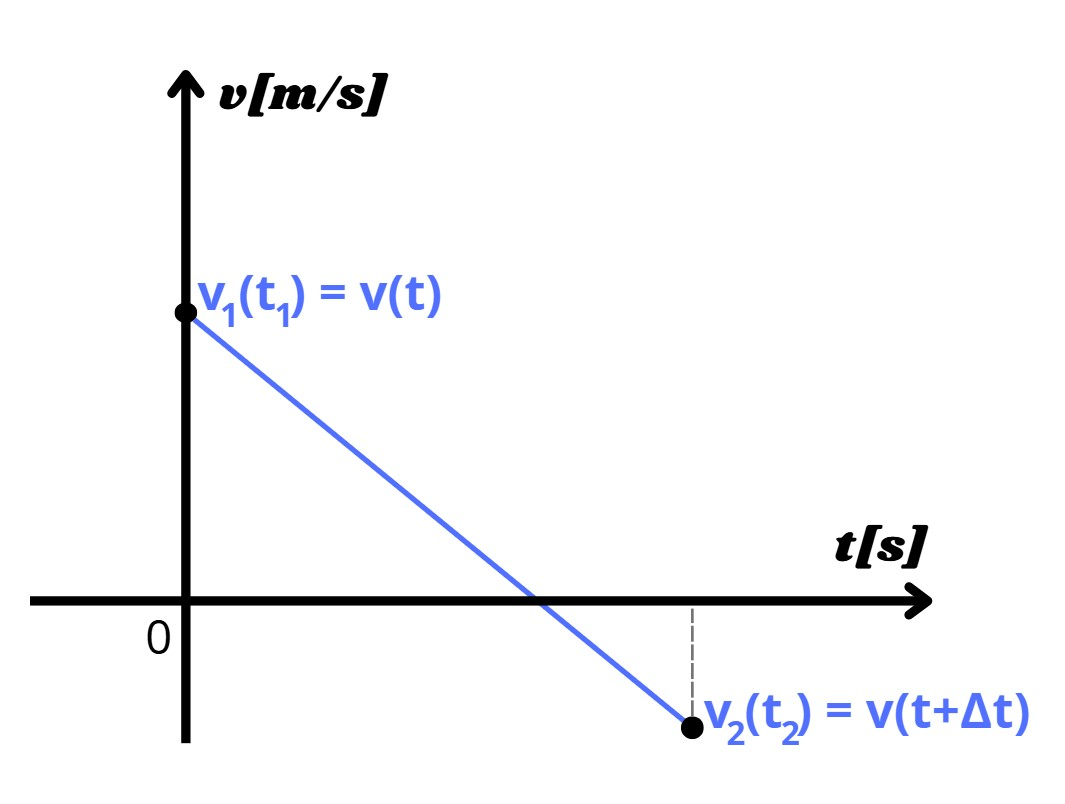
\includegraphics[width=0.6\textwidth]{images/demonstrations/example2.jpg}
    \caption*{Nota: Representación de la aceleración obtenida como derivada de la velocidad respecto al tiempo. }
\end{figure}

\begin{align*}
&\textbf{Comprobación usando integrales:} \\
    a_y &= \lim_{\Delta t \to 0} \frac{v_y(t+\Delta t) - v_y(t)}{\Delta t}
    \quad \text{con } v_{0y}=\text{ctte},\; g=9.8\,\text{m/s}^2 \\
    a_y &= \lim_{\Delta t \to 0} \left(\frac{\Delta v}{\Delta t}\right) \\
    a_y &= \lim_{\Delta t \to 0} \left(\frac{v(t_2) - v(t_1)}{\Delta t}\right) \\
    a_y &= \lim_{\Delta t \to 0} \left(\frac{(v_{0y} - gt_2)-(v_{0y} - gt_1)}{\Delta t}\right) \\
    a_y &= \lim_{\Delta t \to 0} \frac{[v_{0y} - g(t+\Delta t)] - [v_{0y} - gt]}{\Delta t} \\
    a_y &= \lim_{\Delta t \to 0} \frac{\cancel{v_{0y}} - \cancel{gt} - g\Delta t - \cancel{v_{0y}} + \cancel{gt}}{\Delta t} \\
    a_y &= \lim_{\Delta t \to 0} \frac{-g\cancel{\Delta t}}{\cancel{\Delta t}} \\
    a_y &= \lim_{\Delta t \to 0} (-g) \\
    \Aboxed{a_y &= -g} \\
&\textbf{Comprobación usando derivada:} \\
    \vec{a} &= \frac{dv(t)}{dt} \\
    \vec{a} &= \frac{d}{dt}(v_{0y}-gt) \\
    \vec{a} &= \frac{d}{dt}(\cancel{v_{0y}}) - \frac{d}{dt}(gt)\\
    \vec{a} &= -g \cancel{\frac{dt}{dt}}\\
    \Aboxed{a &= -g}
\end{align*}

\input{documentBody/Section4(UniformMovement).tex}
\input{documentBody/Section5(ParticleKinematics).tex}
\section{Cálculo diferencial}

El cálculo diferencial estudia cómo cambian las funciones. Sus herramientas principales son las derivadas, que permiten analizar la variación instantánea de una magnitud.

\subsection{Derivadas}

La derivada de una función mide la tasa de cambio instantánea. Se define como:

\begin{figure}[H]
    \centering
    \captionsetup{width=0.5\textwidth}
    \caption{Interpretación gráfica de la derivada}
    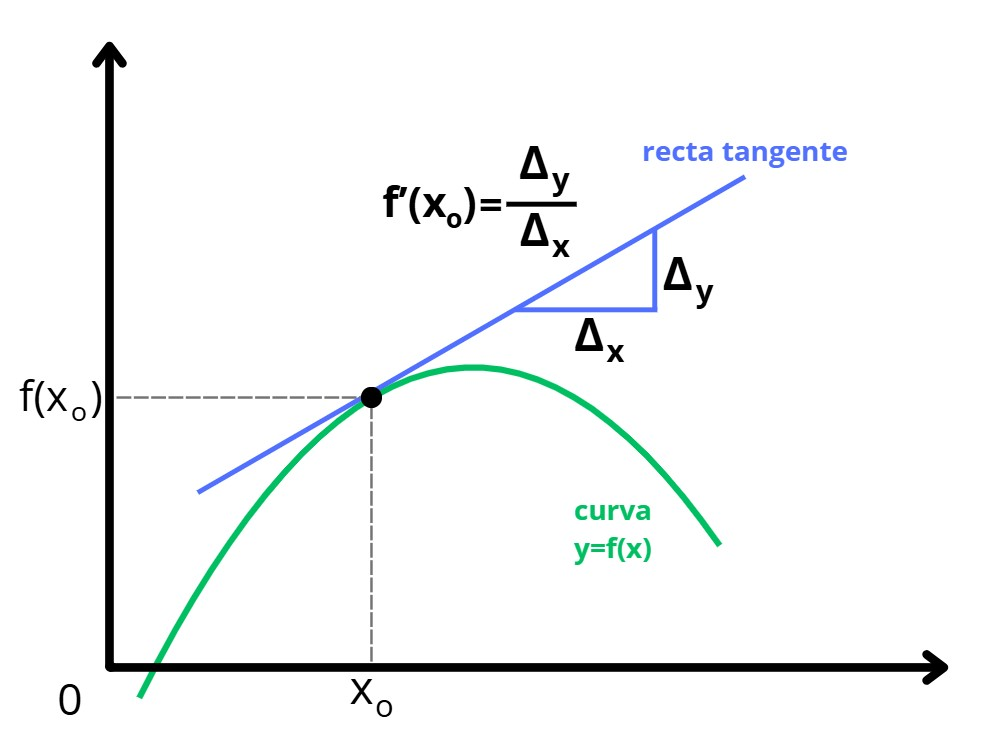
\includegraphics[width=0.6\textwidth]{images/cinematicGraphics/derivative.jpg}
    \caption*{Nota: La derivada se interpreta como la pendiente de la recta tangente a la curva en un punto.}
\end{figure}

\vspace{-40pt}

\[
f'(x) = \lim_{\Delta x \to 0} \frac{f(x+\Delta x) - f(x)}{\Delta x}
\]

\subsubsection{Interpretación}

Geométricamente, la derivada representa la pendiente de la recta tangente a la curva en un punto.

Físicamente, por ejemplo:
\[
v = \frac{dx}{dt}
\]
representa la velocidad como cambio de posición respecto al tiempo.

\subsubsection{Reglas de derivación}

Las reglas de derivación permiten calcular derivadas de manera rápida sin usar directamente la definición.

\begin{itemize}

\item \textbf{Regla de la suma:}

\[
\frac{d}{dx}[f(x) + g(x)] = \frac{df}{dx} + \frac{dg}{dx}
\]

\textbf{Ejemplo:}
\[
\frac{d}{dx}(x^2 + x) = \frac{d}{dx}(x^2) + \frac{d}{dx}(x) = 2x + 1
\]

\item \textbf{Regla del producto:}

\[
\frac{d}{dx}[f(x)g(x)] = f'(x)g(x) + f(x)g'(x)
\]

\textbf{Ejemplo:}
\[
\frac{d}{dx}(x^2 \cdot x) = \frac{d}{dx}(x^2)\cdot x + x^2 \cdot \frac{d}{dx}(x)
\]
\[
= 2x \cdot x + x^2 \cdot 1 = 2x^2 + x^2 = 3x^2
\]

\item \textbf{Regla del cociente:}

% chktex-file 3
\[
\frac{d}{dx}\left[\frac{f(x)}{g(x)}\right] = \frac{f'(x)g(x) - f(x)g'(x)}{g(x)^2}
\]

\textbf{Ejemplo:}
\[
\frac{d}{dx}\left(\frac{x^2}{x}\right)
= \frac{\frac{d}{dx}(x^2)\cdot x - x^2 \cdot \frac{d}{dx}(x)}{x^2}
\]
\[
= \frac{2x \cdot x - x^2 \cdot 1}{x^2}
= \frac{2x^2 - x^2}{x^2} = 1
\]

\item \textbf{Regla de la cadena:}

\[
\frac{d}{dx}f(g(x)) = f'(g(x)) \cdot g'(x)
\]

\textbf{Ejemplo:}
\[
\frac{d}{dx}(x^2 + 1)^2 = \frac{d}{dx}\left[(x^2 + 1)^2\right]
\]
\[
= 2(x^2 + 1)\cdot \frac{d}{dx}(x^2 + 1)
\]
\[
= 2(x^2 + 1)\cdot (2x) = 4x(x^2 + 1)
\]

\end{itemize}

\subsubsection{Derivadas básicas}

\begin{itemize}

\item Potencia:
\[
\frac{d}{dx}(x^n) = nx^{n-1}
\]

\textbf{Ejemplo:}
\[
\frac{d}{dx}(x^3) = 3x^2
\]

\item Seno:
\[
\frac{d}{dx}(\sin x) = \cos x
\]

\item Coseno:
\[
\frac{d}{dx}(\cos x) = -\sin x
\]

\item Exponencial:
\[
\frac{d}{dx}(e^x) = e^x
\]

\end{itemize}

\subsection{Integrales}

La integral es la operación inversa de la derivada y permite calcular áreas bajo la curva.

\subsubsection{Integral indefinida}

\begin{figure}[H]
    \centering
    \captionsetup{width=0.5\textwidth}
    \caption{Interpretación gráfica de la integral indefinida}
    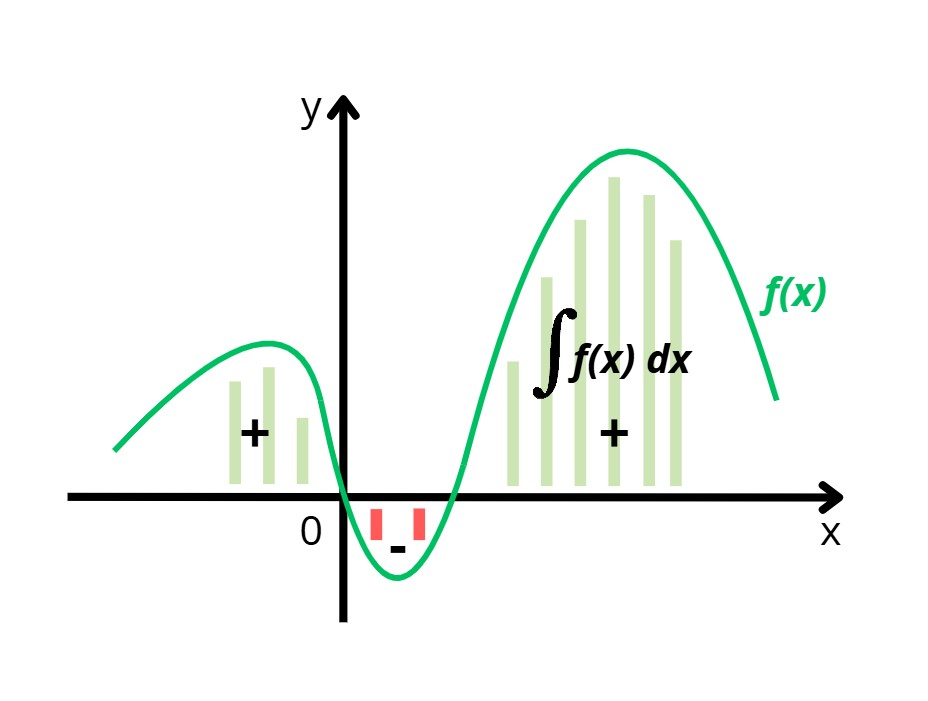
\includegraphics[width=0.6\textwidth]{images/cinematicGraphics/indefiniteIntegral.jpg}
    \caption*{Nota: Familia de funciones cuya derivada es la función dada.}
\end{figure}

\vspace{-40pt}

\[
\int f(x)\,dx = F(x) + C
\]

donde $F'(x) = f(x)$, es decir, $F(x)$ es una función cuya derivada es $f(x)$.

\textbf{Ejemplo:}
\[
\int 2x \, dx = x^2 + C
\]

porque:
\[
\frac{d}{dx}(x^2) = 2x
\]


\subsubsection{Integral definida}

\begin{figure}[H]
    \centering
    \captionsetup{width=0.5\textwidth}
    \caption{Interpretación gráfica de la integral definida}
    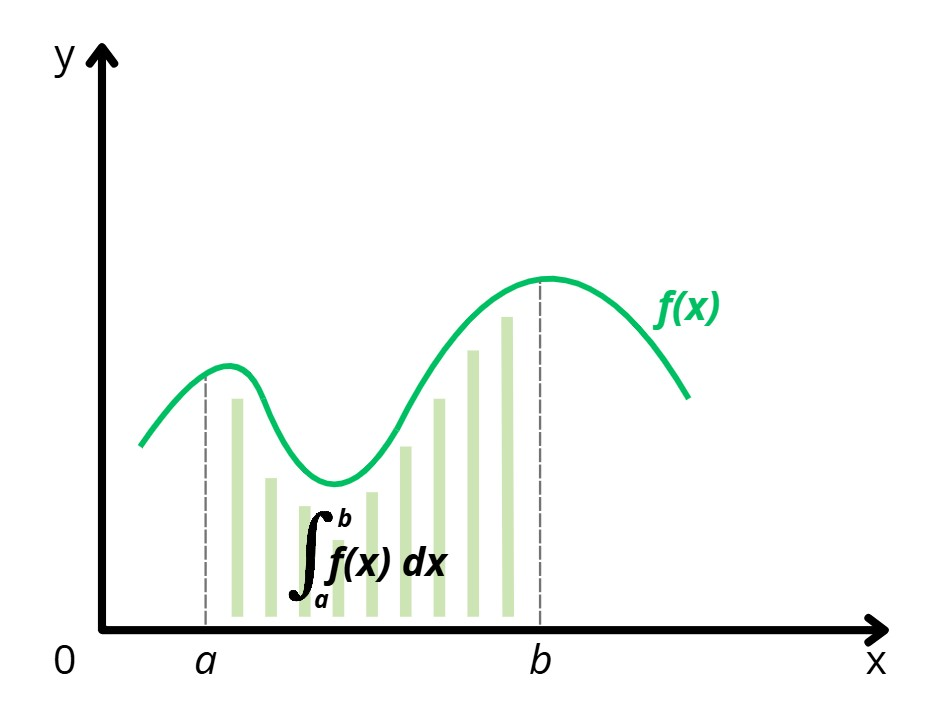
\includegraphics[width=0.6\textwidth]{images/cinematicGraphics/definiteIntegral.jpg}
    \caption*{Nota: Área bajo la curva en un intervalo determinado.}
\end{figure}

\vspace{-40pt}

\[
\int_a^b f(x)\,dx
\]

representa el área bajo la curva entre $a$ y $b$.

\textbf{Ejemplo:}
\[
\int_0^2 x \, dx
\]

Primero encontramos una primitiva:
\[
\int x \, dx = \frac{x^2}{2}
\]

Luego evaluamos en los límites:
\[
\left[\frac{x^2}{2}\right]_0^2 = \frac{2^2}{2} - \frac{0^2}{2}
\]
\[
= \frac{4}{2} - 0 = 2
\]

\subsubsection{Reglas de integración}

\begin{itemize}

\item \textbf{Regla de la potencia:}
\[
\int x^n dx = \frac{x^{n+1}}{n+1} + C
\]

\[
\int x^2 dx = \frac{x^3}{3} + C
\]

\item \textbf{Integral del coseno:}
\[
\int \cos x \, dx = \sin x + C
\]

\item \textbf{Integral del seno:}
\[
\int \sin x \, dx = -\cos x + C
\]

\end{itemize}

\input{documentBody/Section7(MRU).tex}
\input{documentBody/Section8(MRUA).tex}
\input{documentBody/Section9(MVCL).tex}
% !TeX root = ../main.tex
\section{Herramientas}

\subsection{Herramientas para la redacción del informe}

Para la redacción y edición del informe se utilizaron las siguientes herramientas:

% chktex-file 44
\begin{table}[H]
\centering
\begin{tabular}{|p{12cm}|}
\hline
\textbf{1. Canva}
\vspace{-20pt}
\begin{center}
\includegraphics[width=3cm]{images/tools/canva.png}\end{center} \\ \hline
\textbf{Descripción:} Herramienta de diseño gráfico en línea que permite crear presentaciones, infografías y materiales visuales. \\ \hline
\textbf{Uso:} Elaboración y diseño de gráficas \\ \hline
\textbf{Acceso en línea:} \href{https://www.canva.com/design/DAHFYrvBRTM/uSoooPNlrBeWf89NVjZ5Jg/edit}{\textit{Pulsa aquí}} \\
\hline
\end{tabular}
\vspace{10pt}
\caption{Tabla: Herramienta Canva}
\end{table}

\vspace{-20pt}

\begin{table}[H]
\centering
\begin{tabular}{|p{12cm}|}
\hline
\textbf{2. Overleaf}
\vspace{-20pt}
\begin{center}
\includegraphics[width=3cm]{images/tools/overleaf.jpg}\end{center} \\ \hline
\textbf{Descripción:} Plataforma en línea para la edición y compilación de documentos en \LaTeX{}, que permite el trabajo colaborativo en tiempo real. \\ \hline
\textbf{Uso:} Redacción, edición y formato del informe en las etapas iniciales del proyecto \\ \hline
\textbf{Acceso en línea:} \href{https://es.overleaf.com/read/dpqxbgmcnzhv#8991a9}{\textit{Pulsa aquí}} \\
\hline
\end{tabular}
\vspace{10pt}
\caption{Tabla: Herramienta Overleaf}
\end{table}

\vspace{-20pt}

Debido al límite de compilaciones gratuitas de Overleaf, el flujo de trabajo migró hacia un entorno local utilizando GitHub como repositorio y Visual Studio Code como editor principal.

\begin{table}[H]
\centering
\begin{tabular}{|p{12cm}|}
\hline
\textbf{3. GitHub}
\vspace{-20pt}
\begin{center}
\includegraphics[width=3cm]{images/tools/github.png}\end{center} \\ \hline
\textbf{Descripción:} Plataforma de desarrollo colaborativo basada en control de versiones con Git, que permite gestionar y compartir repositorios de código. \\ \hline
\textbf{Uso:} Almacenamiento, control de versiones y colaboración en la redacción del informe \\ \hline
\textbf{Acceso en línea:} \href{https://github.com/AdrianaGut257/Proyecto1}{\textit{Pulsa aquí}} \\
\hline
\end{tabular}
\vspace{10pt}
\caption{Tabla: Herramienta GitHub}
\end{table}

\vspace{-20pt}

\begin{table}[H]
\centering
\begin{tabular}{|p{12cm}|}
\hline
\textbf{4. Visual Studio Code}
\vspace{-20pt}
\begin{center}
\includegraphics[width=3cm]{images/tools/visualStudioCode.png}\end{center} \\ \hline
\textbf{Descripción:} Editor de código desarrollado por Microsoft que soporta múltiples lenguajes de programación y cuenta con funciones de depuración y control de versiones integrado. \\ \hline
\textbf{Uso:} Redacción, edición y compilación local del informe mediante la extensión \textit{LaTeX Workshop} \\ \hline
\textbf{Recurso en línea:} \href{https://code.visualstudio.com/}{\textit{Pulsa aquí}} \\
\hline
\end{tabular}
\vspace{10pt}
\caption{Tabla: Herramienta Visual Studio Code}
\end{table}

\vspace{-20pt}

Para compilar documentos \LaTeX{} localmente desde Visual Studio Code se requiere instalar los siguientes componentes:

\begin{enumerate}
    \setlength{\itemsep}{2pt}
    \item \textbf{MiKTeX} — distribución de \LaTeX{} para Windows: \href{https://miktex.org/download}{\textit{miktex.org/download}}
    \item \textbf{Perl} (Strawberry Perl) — requerido por ciertas extensiones: \href{https://strawberryperl.com/}{\textit{strawberryperl.com}}
    \item \textbf{Extensiones de VS Code:} \textit{LaTeX Workshop} y \textit{LaTeX Utilities}
\end{enumerate}

Se puede seguir el siguiente tutorial para la configuración completa del entorno:
\href{https://www.youtube.com/watch?v=kLT0QVnz3vk&t=1211s}{\textit{Tutorial: configuración de \LaTeX{} en VS Code (YouTube)}}

\vspace{20pt}


\subsection{Herramientas para la presentación de la exposición}
Para la presentación de la exposición se utilizaron las siguientes herramientas:

\begin{table}[H]
\centering
\begin{tabular}{|p{12cm}|}
\hline
\textbf{1. Canva}
\vspace{-20pt}
\begin{center}
\includegraphics[width=3cm]{images/tools/canva.png}\end{center} \\ \hline
\textbf{Descripción:} Herramienta de diseño gráfico en línea que permite crear presentaciones, infografías y materiales visuales. \\ \hline
\textbf{Uso:} Elaboración y diseño de gráficas \\ \hline
\textbf{Acceso en línea:} \href{https://www.canva.com/design/DAHEoMvoq_w/FYudFVc1SgT-2tPS9ydhBQ/edit}{\textit{Pulsa aquí}} \\
\hline
\end{tabular}
\vspace{10pt}
\caption{Tabla: Herramienta Canva}
\end{table}

\vspace{-20pt}

\begin{table}[H]
\centering
\begin{tabular}{|p{12cm}|}
\hline
\textbf{2. Capcut}
\vspace{-20pt}
\begin{center}
\includegraphics[width=3cm]{images/tools/capcut.jpg}\end{center} \\ \hline
\textbf{Descripción:} Herramienta de edición de video en línea que permite crear videos creativos con efectos y transiciones. \\ \hline
\textbf{Uso:} Edición y producción de videos para la presentación de la exposición \\ \hline
\textbf{Recurso en línea:} \href{https://www.capcut.com/}{\textit{Pulsa aquí}} \\
\hline
\end{tabular}
\vspace{10pt}
\caption{Tabla: Herramienta Capcut}
\end{table}

\vspace{-20pt}

\begin{table}[H]
\centering
\begin{tabular}{|p{12cm}|}
\hline
\textbf{3. Audacity}
\vspace{-20pt}
\begin{center}
\includegraphics[width=3cm]{images/tools/audacity.png}\end{center} \\ \hline
\textbf{Descripción:} Software de edición de audio que permite grabar, editar y mejorar archivos sonoros. \\ \hline
\textbf{Uso:} Edición y mejora del audio utilizado en la presentación \\ \hline
\textbf{Recurso en línea:} \href{https://www.audacityteam.org/}{\textit{Pulsa aquí}} \\
\hline
\end{tabular}
\vspace{10pt}
\caption{Tabla: Herramienta Audacity}
\end{table}

\vspace{-20pt}

Para complementar la presentación, se emplearon diversos recursos multimedia:

\begin{itemize}
    \item \textbf{Videos:} obtenidos de \href{https://www.pexels.com/}{\textit{www.pexels.com}}
    \item \textbf{Efectos de audio:} obtenidos de \href{https://freesound.org/}{\textit{freesound.org}}
    \item \textbf{Música de fondo:} \textit{Handel: Passacaglia | Metamorphose String Orchestra}
\end{itemize}

\subsection{Herramientas para la simulación}
Para la simulación se utilizaron las siguientes herramientas:

\begin{table}[H]
\centering
\begin{tabular}{|p{12cm}|}
\hline
\textbf{1. GeoGebra}
\vspace{-20pt}
\begin{center}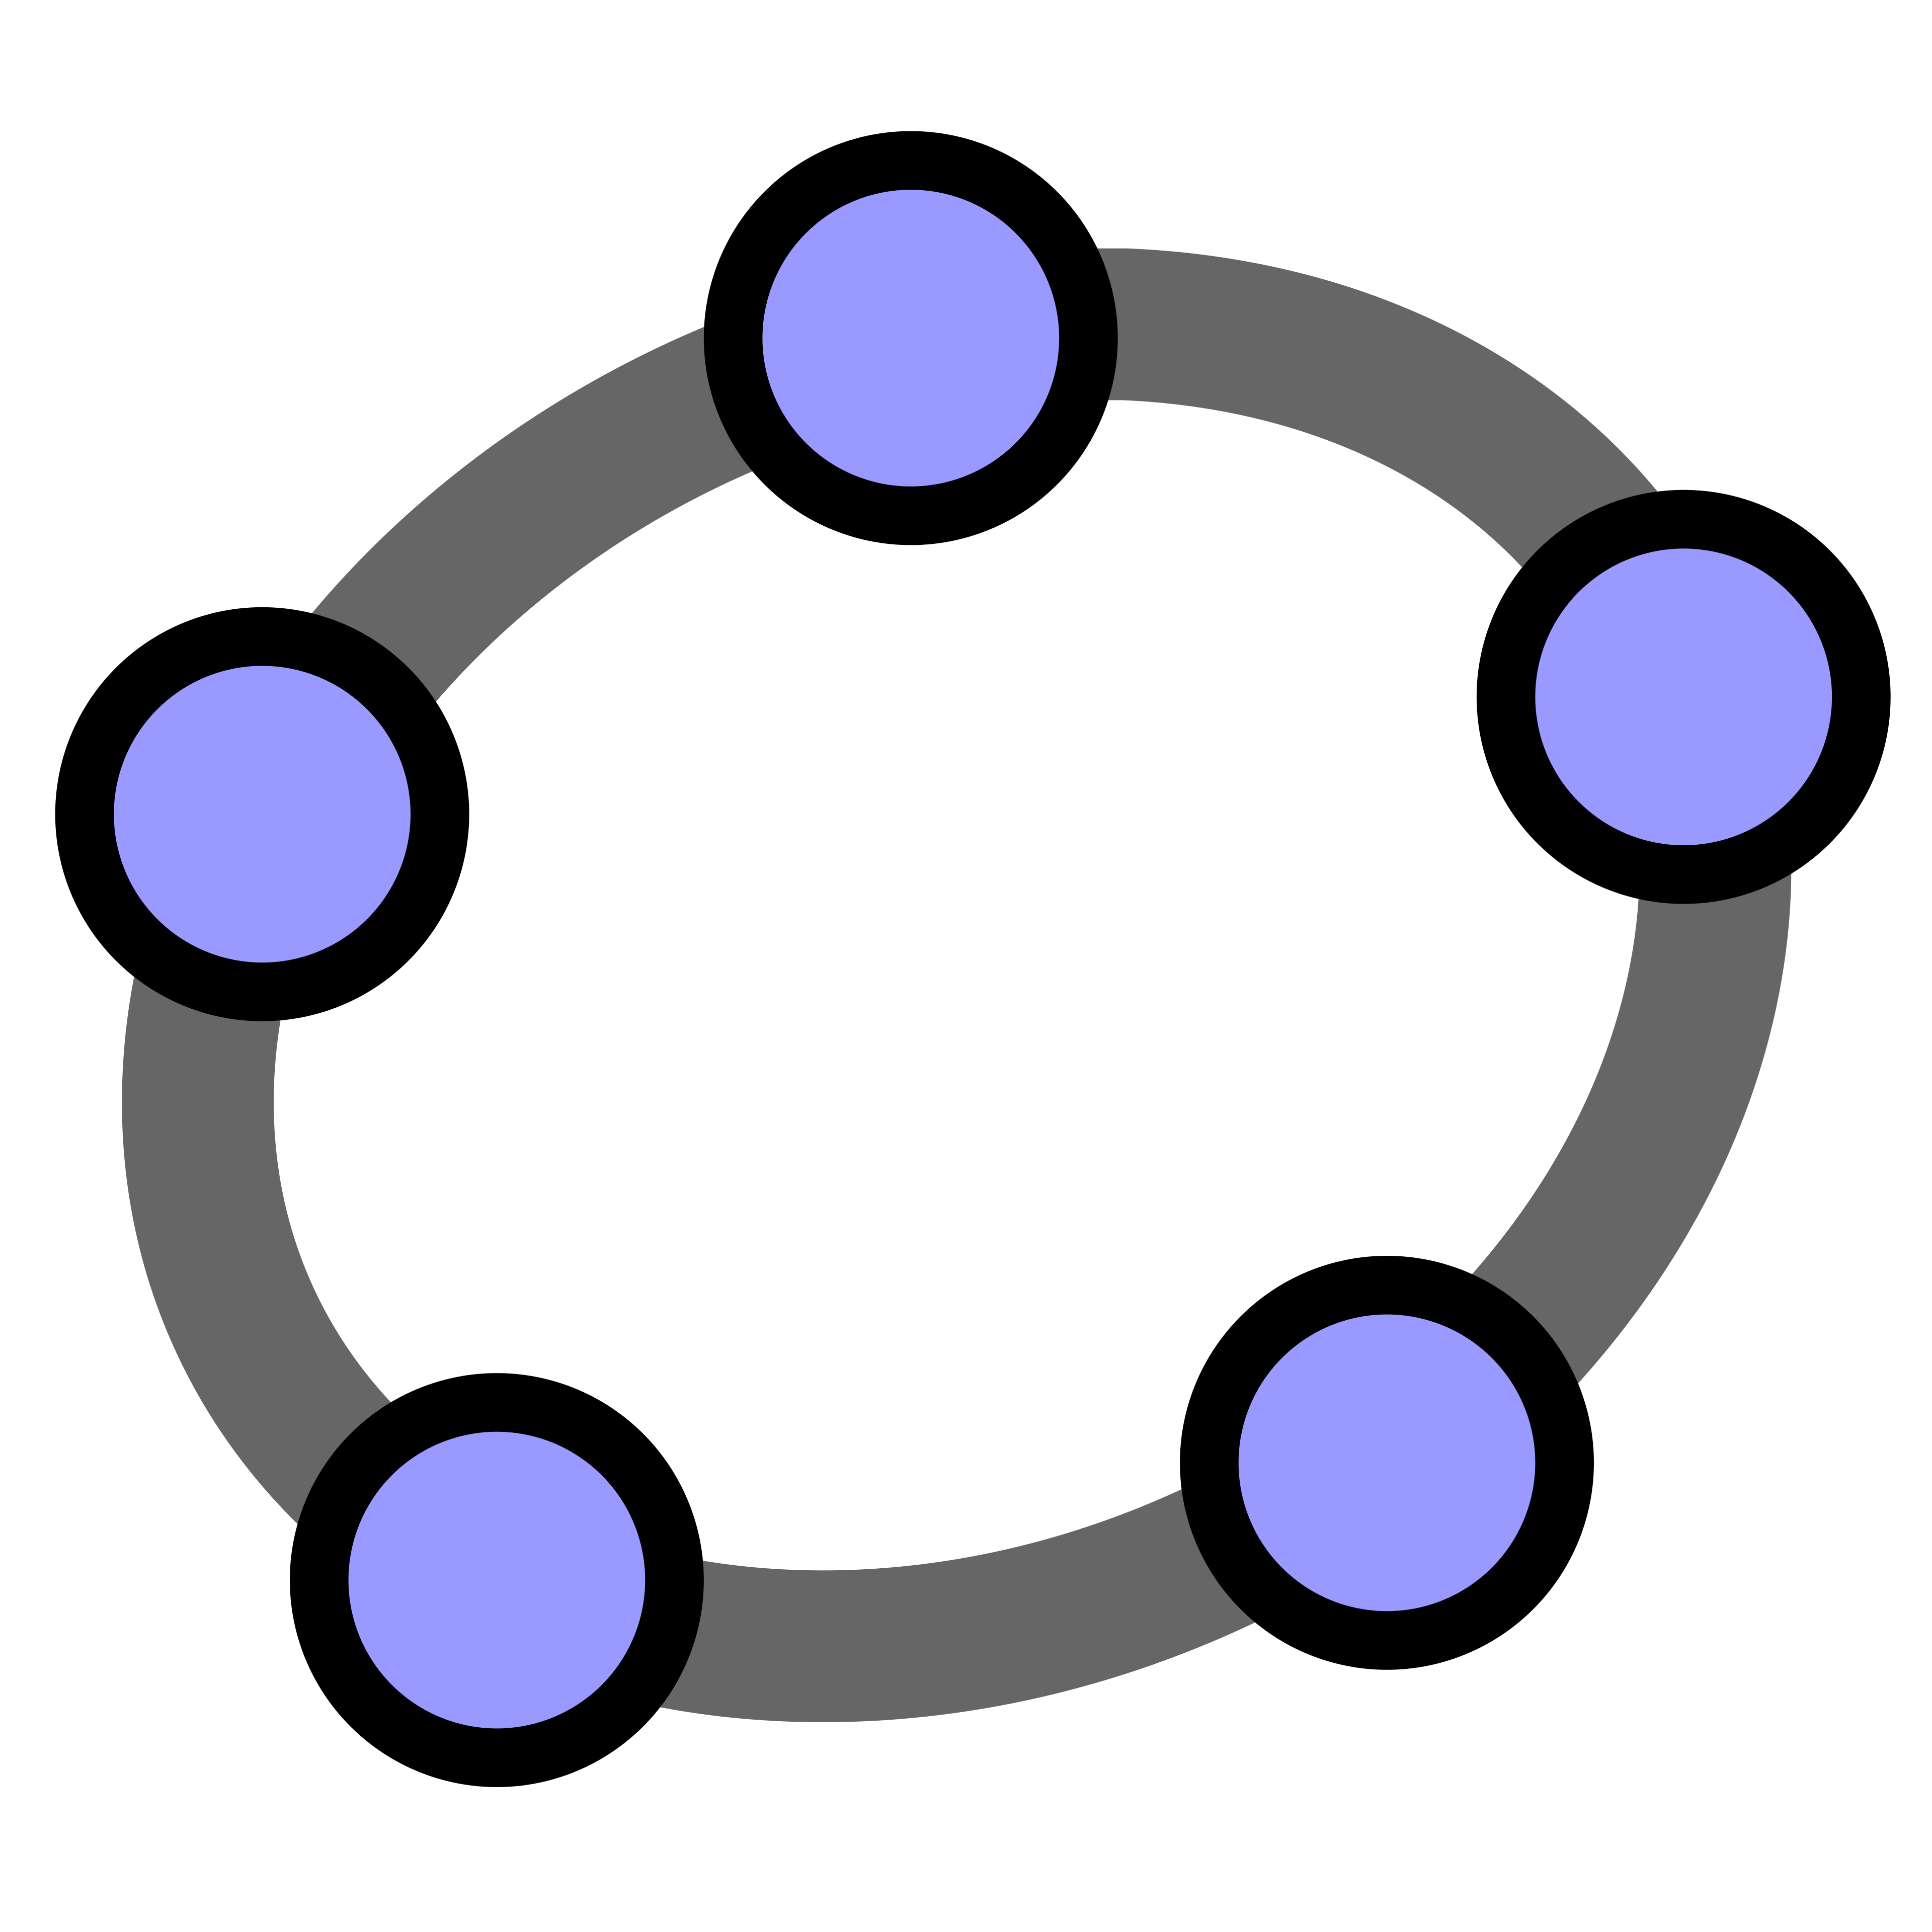
\includegraphics[width=3cm]{images/tools/geogebra.png}\end{center} \\ \hline
\textbf{Descripción:} Software matemático dinámico que permite representar gráficamente funciones, realizar construcciones geométricas y analizar fenómenos algebraicos y de cálculo. \\ \hline
\textbf{Uso:} Visualización de gráficas para la simulación \\ \hline
\textbf{Recurso en línea:} \href{https://www.geogebra.org/?lang=es}{\textit{Pulsa aquí}} \\
\hline
\end{tabular}
\vspace{10pt}
\caption{Tabla: Herramienta GeoGebra}
\end{table}

\vspace{-20pt}
\section{Simulación}

\subsection{Materiales}

\begin{itemize}
    \item Computadora o laptop
    \item Software GeoGebra
    \item Cuaderno de apuntes
    \item Calculadora científica
\end{itemize}

\subsection{Procedimiento}

\begin{enumerate}
    \item Abrir el software GeoGebra.
    \item En la barra de entrada, definir la función de posición del automóvil (MRU):
    \[
    x_a(t) = 40t
    \]
    \item Definir la función de posición del camión (MRUA):
    \[
    x_c(t) = 2t^2 + 80
    \]
    \item Observar las curvas generadas: la del automóvil es una línea recta y la del camión es una parábola.
    \item Identificar gráficamente los puntos de intersección entre ambas curvas.
    \item Verificar los resultados obtenidos analíticamente con los valores leídos en la gráfica.
\end{enumerate}

El ejercicio simulado es el siguiente:

\textbf{Un automóvil se mueve a velocidad constante de 144 km/h en una carretera recta. En determinado momento, un camión que está a 80 m delante del automóvil comienza a moverse desde el reposo con una aceleración de 4 m/s$^2$. Determinar:}
\begin{itemize}
    \item[{a)}] El tiempo y la posición cuando el automóvil y el camión se encuentran juntos.
    \item[{b)}] El momento cuando la velocidad del automóvil y del camión son iguales, y la separación entre ellos en ese instante.
\end{itemize}

\subsection{Resolución}

\textbf{Datos del problema:}

\begin{itemize}
    \item \textbf{Automóvil:}
    \begin{align*}
        v_a &= 144\,\frac{\cancel{\text{km}}}{\cancel{\text{h}}} \cdot \frac{1000\,\text{m}}{1\,\cancel{\text{km}}} \cdot \frac{1\,\cancel{\text{h}}}{3600\,\text{s}} = 40\,\frac{\text{m}}{\text{s}} \\
        x_{0a} &= 0\,\text{m} \\
        a_a &= 0\,\frac{\text{m}}{\text{s}^2}
    \end{align*}

    \item \textbf{Camión:}
    \begin{align*}
        v_{0c} &= 0\,\frac{\text{m}}{\text{s}} \\
        x_{0c} &= 80\,\text{m} \\
        a_c &= 4\,\frac{\text{m}}{\text{s}^2}
    \end{align*}
\end{itemize}

\textbf{Velocidad del camión (MRUA):}
\vspace{-20pt}

\begin{align*}
a_c &= \frac{dv}{dt} \\
4 &= \frac{dv}{dt} \\
dv &= 4\,dt \\
\int_{0}^{v} dv &= \int_{0}^{t} 4\,dt \\
\left[v\right]_{0}^{v} &= 4\left[t\right]_{0}^{t} \\
v - 0 &= 4(t - 0) \\
\Aboxed{v_c &= 4t}
\end{align*}

\textbf{Posición del camión (MRUA):}
\vspace{-20pt}

\begin{align*}
v_c &= \frac{dx}{dt} \\
4t &= \frac{dx}{dt} \\
dx &= 4t\,dt \\
\int_{80}^{x} dx &= \int_{0}^{t} 4t\,dt \\
\left[x\right]_{80}^{x} &= 2\left[t^2\right]_{0}^{t} \\
x - 80 &= 2(t^2 - 0) \\
x - 80 &= 2t^2 \\
\Aboxed{x_c &= 2t^2 + 80}
\end{align*}

\textbf{Posición del automóvil (MRU):}
\vspace{-20pt}

\begin{align*}
v_a &= \frac{dx}{dt} \\
40 &= \frac{dx}{dt} \\
dx &= 40\,dt \\
\int_{0}^{x} dx &= \int_{0}^{t} 40\,dt \\
\left[x\right]_{0}^{x} &= 40\left[t\right]_{0}^{t} \\
x - 0 &= 40(t - 0) \\
\Aboxed{x_a &= 40t}
\end{align*}

\subsubsection*{a) Tiempo y posición cuando se encuentran juntos}

Para que el automóvil y el camión estén en la misma posición, igualamos sus ecuaciones de posición:
\vspace{-20pt}

\begin{align*}
x_a &= x_c \\
40t &= 2t^2 + 80 \\
0 &= 2t^2 - 40t + 80 \\
0 &= t^2 - 20t + 40
\end{align*}

Aplicando la fórmula general:
\vspace{-20pt}

\begin{align*}
t &= \frac{-b \pm \sqrt{b^2 - 4ac}}{2a} \\
t &= \frac{20 \pm \sqrt{(-20)^2 - 4(1)(40)}}{2(1)} \\
t &= \frac{20 \pm \sqrt{400 - 160}}{2} \\
t &= \frac{20 \pm \sqrt{240}}{2} \\
t &= \frac{20 \pm 15{,}49}{2}
\end{align*}

Se obtienen dos eventos:
\vspace{-20pt}

\[
\textbf{Primer evento:} \quad t_1 = \frac{20 - 15{,}49}{2} = \frac{4{,}51}{2} \approx 2{,}25\,\text{s} \Rightarrow t_1 \approx 2{,}3\,\text{s}
\]

\[
\textbf{Segundo evento:} \quad t_2 = \frac{20 + 15{,}49}{2} = \frac{35{,}49}{2} \approx 17{,}74\,\text{s}
\]

\textit{Nota: El primer evento ($t_1 \approx 2{,}3$ s) es físicamente el relevante; corresponde al momento en que el auto alcanza al camión por primera vez.}

Calculando la posición en $t_1 \approx 2{,}3$ s:

\begin{align*}
x_a &= 40t_1 = 40(2{,}25) = 90\,\text{m} \\
x_c &= 2(2{,}25)^2 + 80 = 2(5{,}0625) + 80 = 10{,}125 + 80 \approx 90{,}2\,\text{m}
\end{align*}

\[
\boxed{t_1 \approx 2{,}3\,\text{s}, \qquad x \approx 90{,}2\,\text{m}}
\]

\subsubsection*{b) Momento en que las velocidades son iguales y separación}

\vspace{-40pt}

\begin{align*}
\intertext{Igualamos la velocidad del automóvil con la del camión:}
v_a &= v_c \\
40 &= 4t \\
t &= \frac{40}{4} \\
\Aboxed{t &= 10\,\text{s}}
\intertext{Evaluamos las posiciones en $t = 10$ s:}
x_a &= 40t = 40(10) = 400\,\text{m} \\
x_c &= 2t^2 + 80 = 2(10)^2 + 80 = 200 + 80 = 280\,\text{m}
\intertext{Separación entre ellos:}
\Delta x &= x_a - x_c \\
\Delta x &= 400 - 280 \\
\Aboxed{\Delta x &= 120\,\text{m}}
\end{align*}

\subsection{Resultados}

A partir de la simulación realizada en GeoGebra se obtuvieron los siguientes resultados:

\begin{itemize}
    \item La gráfica del automóvil es una línea recta (MRU), con pendiente constante igual a su velocidad (40 m/s).
    \item La gráfica del camión es una parábola (MRUA), que parte desde $x = 80$ m y se acelera progresivamente.
    \item Las dos curvas se intersectan en dos puntos: el primero alrededor de $t \approx 2{,}3$ s y el segundo en $t \approx 17{,}74$ s.
\end{itemize}

\begin{table}[H]
\centering
\begin{tabular}{c|c|c|c}
Tiempo (s) & $x_{\text{auto}}$ (m) & $x_{\text{camión}}$ (m) & $v_{\text{camión}}$ (m/s) \\\hline
0   & 0     & 80    & 0  \\
2{,}3 & 90  & 90{,}2 & 9{,}2 \\
5   & 200   & 130   & 20 \\
10  & 400   & 280   & 40 \\
17{,}74 & 709{,}6 & 709{,}6 & 70{,}96 \\
\end{tabular}
\caption{Datos obtenidos en la simulación}
\end{table}

\vspace{-20pt}

\subsection{Análisis}

Los resultados obtenidos permiten observar que:

\begin{itemize}
    \item El automóvil, al tener mayor velocidad inicial, alcanza rápidamente al camión en $t \approx 2{,}3$ s (posición $\approx 90{,}2$ m). Sin embargo, como el camión está acelerando, eventualmente lo supera, por lo que el automóvil vuelve a alcanzarlo en el segundo evento ($t \approx 17{,}74$ s).
    \item En $t = 10$ s las velocidades son iguales (ambas 40 m/s), pero el camión aún está 120 m por detrás del automóvil. A partir de ese momento, el camión, al seguir acelerando, comenzará a reducir esa brecha.
    \item La diferencia en el tipo de movimiento (MRU vs MRUA) genera dos intersecciones en la gráfica posición-tiempo, lo cual tiene un significado físico claro: primero el auto pasa al camión, y luego el camión recupera y alcanza al auto.
\end{itemize}
\input{documentBody/Section12(Conclusions).tex}
\input{documentBody/Section13(Recommendations).tex}

%%%%%%%%%%%%%%%%%%
%  BIBLIOGRAFÍA  %
%%%%%%%%%%%%%%%%%%
\nocite{*}
\printbibliography[title={Bibliografía}]

\end{document}